\documentclass[10pt,conference,compsocconf]{IEEEtran}

%\usepackage{times}
%\usepackage{balance}
\usepackage{url}
\usepackage{xcolor}
\usepackage{graphicx}	% For figure environment
\usepackage{amsmath}
\usepackage{amsfonts}
\usepackage{hyperref}
\usepackage{tikz}
\usetikzlibrary{shapes.geometric, arrows.meta, positioning}

\begin{document}
\title{LightGCN+ \\ A Graph Convolutional Network for Matrix Completion}

\author{
  Alain Joss \\
  Solomon Thiessen \\
  Antoine Suter \\
  Department of Computer Science, ETH Zurich, Switzerland
}

\maketitle

\begin{abstract}
  Personalized recommendation systems are critical for businesses aiming to enhance user experience and satisfaction. In this study, we address the task of collaborative filtering through the lens of matrix completion. While the primary objective of collaborative filtering is to rank preferences for unobserved user-item interactions, accurate rating predictions can offer deeper insights into user preferences, thereby informing better decision-making across various use cases.
  
  In this work, we propose LightGCN+, an advanced graph convolutional encoder-decoder model that extends the original LightGCN architecture. Whereas LightGCN was primarily designed for item recommendation through ranking, LightGCN+ is tailored to predict real-valued ratings.
  LightGCN+ leverages the graph convolutional framework of LightGCN, modified to handle real-valued rating matrices. Additionally, we introduce a multi-layer perceptron (MLP) at the decoder stage.
  Our approach proves to be robust, achieving comparable performance to state-of-the-art models.
\end{abstract}

\section{Introduction}
Collaborative filtering (CF) is a widely used approach in recommendation systems that leverages historical user-item interactions to predict future preferences \cite{koren2009matrix}. The core idea is to exploit patterns in the collective behavior of users to make personalized recommendations. A common formulation of CF is as a matrix completion problem, where the goal is to predict missing entries in a sparse user-item interaction matrix \cite{candès2009exact}.
Traditional matrix factorization techniques like singular value decomposition have been successful for CF \cite{koren2009matrix}. More recently, deep learning approaches have achieved state-of-the-art performance on CF tasks. Models like Neural Collaborative Filtering \cite{he2017neural} and Deep Matrix Factorization \cite{xue2017deep} use neural networks to learn nonlinear latent representations.
Graph-based models have emerged as a powerful paradigm for CF by naturally representing user-item interactions as a bipartite graph \cite{berg2017graph}. Graph Convolutional Networks (GCNs) in particular have shown promising results by leveraging higher-order connectivity information \cite{ying2018graph}. LightGCN \cite{he2020lightgcn} simplified the GCN architecture for recommendation by removing feature transformation and nonlinear activation, demonstrating strong performance with a lightweight design.
In this work, we propose LightGCN+, an extension of LightGCN tailored for explicit rating prediction rather than ranking. While LightGCN focuses on binary interactions, LightGCN+ is designed to handle real-valued rating matrices. We modify the graph convolution operation to incorporate rating information and introduce a multi-layer perceptron decoder to predict continuous ratings. This allows our model to capture fine-grained user preferences beyond just positive interactions.
The key contributions of this work are:
\begin{itemize}
\item We extend LightGCN to handle explicit rating prediction for collaborative filtering.
\item We propose a novel graph convolution formulation that leverages rating information.
\item We introduce a flexible decoder architecture to map latent representations to ratings.
\item We demonstrate competitive performance compared to state-of-the-art rating prediction models.
\end{itemize}
The rest of this paper is organized as follows: Section 2 describes our proposed LightGCN+ model in detail. Section 3 presents the experiments conducted on the ETHZ-CIL-Collaborative-Filtering-2024 dataset. 
Section 4 discusses results, and Section 5 concludes the paper.

\section{Model and Methods}
\subsection{Problem Formulation}
Given a sparse user-item rating matrix $R \in \mathcal{R}^{m \times n}$, with observed ratings $r_{u,i}$ for observed interaction pairs $(u,i) \in \Omega$, the task of matrix completion consists of predicting the missing ratings in $R$.

Graph based methods approach matrix completion by representing the user-item interactions as a bipartite graph $G = (U, I, E)$, where $U$ and $I$ are the sets of users and items (nodes), respectively, and $E$ is the set interactions (edges) with weights $r_{u,i}$.
The adjacency matrix $A \in \mathcal{R}^{(m+n) \times (m+n)}$ of the bipartite graph $G$ is defined as:
\begin{equation}
    A = \begin{bmatrix}
    0 & R \\
    R^T & 0
    \end{bmatrix}
\end{equation}
The adjacency matrix may be preprocessed using different normalization techniques.
We define the standardized adjacency matrix \(\hat{A}\) as:
\begin{equation}
    \hat{A} = \begin{bmatrix}
    0 & Z_{\text{col}} \\
    Z_{\text{row}}^T & 0
    \end{bmatrix}
    \label{eq:A_hat}
\end{equation}
where \(Z_{\text{col}}\) and \(Z_{\text{row}}\) represent the standardized user-item ratings, derived using z-score normalization on the columns and rows of \(R\), respectively. 

\subsection{Model Architecture}
The LightGCN+ model consists of an encoder-decoder architecture, with the encoder comprising a multi-layer graph convolutional network and an aggregation function, and the decoder consisting of a multi-layer perceptron (MLP).

Users and items are represented by node embeddings $e_v \in \mathbb{R}^K$, for all $v \in U \cup I$, which are learned during training.

\subsection{Encoder}
The encoder of LightGCN+ takes the embedding matrix $E \in R^{(m+n)\times K}$ and the standardized adjacency matrix \(\hat{A}\) as inputs, and generates hidden representations $H$, which are then passed to the decoder.

\subsubsection{Graph Convolution}
Graph convolution is a form of message passing over the graph, where each node updates its representation by aggregating information from its neighbors, reflecting the local graph structure. 
Applying this operation multiple times, in a layered fashion, enables the model to capture higher-order relationships between nodes.
For a given node $v$, the hidden representation $h_v^{(l+1)}$ at layer $l+1$ is computed as:
\begin{align}
    h_u^{(l+1)} &= \sum_{i \in N(u)} \frac{z_{\text{col}_{u,i}}}{\sqrt{|N(u)||N(i)|}} h_i^{(l)} \quad \forall u \in U \\
    h_i^{(l+1)} &= \sum_{u \in N(i)} \frac{z_{\text{row}_{u,i}}}{\sqrt{|N(u)||N(i)|}} h_u^{(l)}  \quad \forall i \in I
\end{align}
where $N(v)$ is the set of neighbors of $v$.
Finally, the symmetrical normalization term $\sqrt{|N(u)||N(i)|}$ ensures that the hidden representations are scaled appropriately.
Note that the hidden representations $h_v^{(0)}$ at the input layer correspond to the learnable embeddings $e_v$.

The $L$-layered convolution operation can be expressed more compactly as:
\begin{equation}
    H^{(l+1)} = \tilde{A} H^{(l)}
\end{equation}
where $\tilde{A} = D^{-\frac{1}{2}} \hat{A} D^{-\frac{1}{2}}$ is the normalized standardized-adjacency matrix, $D$ is the diagonal degree matrix of $\hat{A}$, and $H^{(l)}$ is the matrix of hidden representations at layer $l$.

\subsubsection{Aggregation}
After $L$ layers of graph convolution, the hidden representations $h_v^{(l)}$ of node $v$ are aggregagated to obtain the final representations.
In contrast to the original LightGCN model, instead of averaging we use concatentation as aggregation function:
\begin{equation}
    h_v = \oplus(h_v^{(0)}, h^{(1)}, \ldots, h_v^{(L)}) \in \mathbb{R}^{K \cdot (L+1)}
\end{equation}
where $\oplus$ denotes concatenation operator.
Concatentating layered representations is a natural choice of aggregation for LightGCN+, given the use of a multi-layer perceptron (MLP) as the decoder.

\subsection{Decoder}
The decoder of LightGCN+ is a multi-layer perceptron (MLP) that takes the concatenated hidden representations \( h_u \) and \( h_i \) for a user-item pair \((u, i)\) and outputs the predicted rating \(\hat{r}_{u,i}\):
\begin{equation}
    \hat{r}_{u,i} = \text{MLP}(\oplus(h_u, h_i))
\end{equation}
During training, user-item pairs \((u, i) \in \Omega\) (the set of observed interactions), while during inference, \((u, i) \notin \Omega\).

\subsection{Objective Function}
A natural choice of loss function for rating prediction is the mean squared error (MSE) between the predicted ratings \(\hat{R}\) and the true ratings \(R\):
\begin{equation}
    \mathcal{L} = \frac{1}{|\Omega|} \sum_{(u,i) \in \Omega} (\hat{r}_{u,i} - r_{u,i})^2
\end{equation}
Other loss functions could be used, depending on the specific use case.
Learnable parameters of the model include user and item embeddings and the parameters of the MLP.

\section{Experiments}

\subsection{Dataset}

We evaluate the performance of LightGCN+ on the ETHZ-CIL-Collaborative-Filtering-2024 dataset.
The dataset consists of $10,000$ users and $1,000$ items, with $1176952$ observed ratings, which corresponds to a sparsity of $88.23 \%$.
The ratings are integers in the range $[1, 5]$, with a mean rating of $3.86$ and a standard deviation of $1.12$.

\subsection{Preprocessing}
We find that normalizing the $\hat{A}$ using $Z_{\text{col}}$ and $Z_{\text{row}}$, as shown in Equation \ref{eq:A_hat}, significantly enhances the model's generalization ability. 
The rationale behind this dual standardization is that it reduces biases and variances from individual user or item rating patterns. This makes them comparable across the graph, which is crucial for the effectiveness of the convolution operation.

\subsection{Training}
The model is trained end-to-end using the Adam optimizer.
We avoid mini-batching to ensure that the model can learn the global structure of the graph, while also speeding up convergence. 
To prevent overfitting we tuned $\lambda$ and $p$ accordingly. 
We initialize the embeddings using a normal distribution with tunable standard deviation $\sigma_{\text{init}}$, and the MLP weights using Xavier initialization \cite{glorot2010understanding}.
Different models are trained for different amounts of epochs, ranging between $1000$ and $5000$, saving the model with best validation score.

\subsection{Model Design Choices}
During the design phase of the model we conduct several experiments to determine the best architecture for LightGCN+.
\subsubsection{Graph Convolution}
To normalize $\hat{A}$, we follow the standard GCN \cite{kipf2017semi} approach, using the symmetric normalization term $\sqrt{|N(u)||N(i)|}$.
\subsubsection{Layer Aggregation}
We verify the hypothesis that concatenation is a better choice of aggregation function than averaging, both by averaging using equal weights $\alpha^{(l)} = 1/(L+1)$ and by learning the weights $\alpha^{(l)}$.
We also experiment with graph attention \cite{velivckovic2018graph}, to learn the weights $\alpha_{u,i}^{(l)}$ for each user-item pair.
We find that attention performs best with $L=1$, but does not enhance model performance.
\subsubsection{MLP Architecture}
We find that the choice of activation function and hidden layer sizes has a significant impact on the model's performance.
Thus, we leave the MLP architecture to be determined entirely in the hyperparameter tuning phase. However, we decide to use dropout, following the results of \cite{berg2017graph}.
% here we have the answer why attention didn't work, because we have to message pass using attention, not using attention after message passing


\subsection{Hyperparameter Tuning}
To get an approximation of the individual hyperparameters' impact on the model's performance, we perform an initial grid-search over the following ranges:
\begin{itemize}
  \item Initialization standard deviation $\sigma_{\text{init}} \in [0.01, 0.1]$
  \item Learning rate $\eta \in [0.001, 0.1]$
  \item Weight decay $\lambda \in [1e-5, 1e-3]$
  \item Dropout rate $p \in [0.1, 0.7]$
  \item Activation function $f \in$ \{ReLU, LeakyReLU, GELU\}
  \item Number of convolutional layers $L \in [1, 10]$
  \item Embedding dimension $K \in [24, 38]$
  \item MLP hidden layer sizes $C$: \\ $\{(12K,6K), (10K,5K), (8K,4K), (4K,2K)\}$
\end{itemize}

To narrow down the search space, we set the activation function to GELU, as it consistently outperforms other activation functions, and perform a second grid search over different values for $\sigma_{\text{init}}$, $\eta$, $\lambda$, $p$, and $f$, 
testing them on a simple working model $L=4$, $K=32$, and $C=(8K,4K)$.

Finally, we tune the remaining and most impactful hyperparameters in the following ranges:
\begin{itemize}
    \item Embedding dimension $K \in [16, 32]$
    \item Number of convolutional layers $L \in [1, 6]$
    \item MLP hidden layer sizes $[K, 2K, 1]$
\end{itemize}
We find that multiple models with different hyperparameters can achieve similar performance, but there is a clear range of best performing hyperparameters.

\subsection{LightGCN++}
We take advantage of the insights gained in the tuning phase of the base model, defining a LightGCN++ model, which ensembles the top $M$ performing LightGCN+ models of the grid search.
We find that this additional step makes predictions more robust and improves the overall performance of the model.

The ensembled prediction matrix is obtained by computing a weighted average of the predictions of the individual models:
\begin{equation}
    \hat{R} = \sum_{m=1}^{M} w_m \hat{R}_m
\end{equation}
The ensemble weights $w_m$ are determined by splitting the original validation set used during training, into a set for fitting the ensemble weights and a set for evaluating the ensemble's performance.
To prevent overfitting we cap the number of models in the ensemble at $M=10$.




\section{Results}
\label{sec:results}

\label{sec:tips-writing}
Our results, summarized in Table \ref{table:results}, compare the performance of various configurations of LightGCN+, including the LightGCN+ ensemble, against two baseline models: Neural Collaborative Filtering (NCF) and Alternating Least Squares (ALS). We use the root mean squared error (RMSE) as the evaluation metric.

\begin{table}[h!]
  \centering
  \begin{tabular}{l c} 
   \hline
   \textbf{Model} & \textbf{RMSE Score} \\ [0.5ex] 
   \hline
   LightGCN+ Ensemble & 0.9780 \\ 
   LightGCN+ Multilayer (L = 3) & 0.9839 \\ 
   LightGCN+ Single-layer (L = 1) & 0.9871 \\ 
   NCF & 1.0940 \\ 
   ALS & 1.4260 \\ 
   \hline
   \end{tabular}
   \caption{Model performance comparison}
   \label{table:results}
  \end{table}
  
\subsection{LightGCN+}
The LightGCN+ variants significantly outperformed the baseline models, even with a single convolutional layer. 
Performance improved further with the addition of multiple convolutional layers, with the highest performance achieved by models with $L=4, 5, 6$.
The optimal embedding dimension $K$ was found to be around $K=28, 30$. Models with higher $K$ values tended have unstable training runs and overfit fast to the training data.
The MLP architecture was found to have a significant impact on performance, with a two-layer MLP with hidden layer sizes $[12K, 6K]$ performing best.
Adding hidden layers to the MLP did not improve performance, and led to overfitting. Increasing the hidden layer sizes lead to the same result.

The LightGCN++ ensemble model achieved the best performance, demonstrating the effectiveness of ensembling multiple models.

The highest-performing model was trained with the following hyperparameters:
\begin{itemize}
  \item Embedding dimension $K = 28$
  \item Number of convolutional layers $L = 5$
  \item MLP hidden layers sizes = $[12K, 6K, 1]$
  \item Initialization standard deviation: $\sigma_{\text{init}}=0.075$
  \item Learning rate: $\eta=0.01$
  \item Weight decay: $\lambda=5e-5$
  \item Dropout: $p=0.5$
  \item MLP activation function: GELU
\end{itemize}

These parameters are also the once which stabilize most the training process, as shown in Figure \ref{fig:top-model}.
\begin{figure}[h]
  \centering
  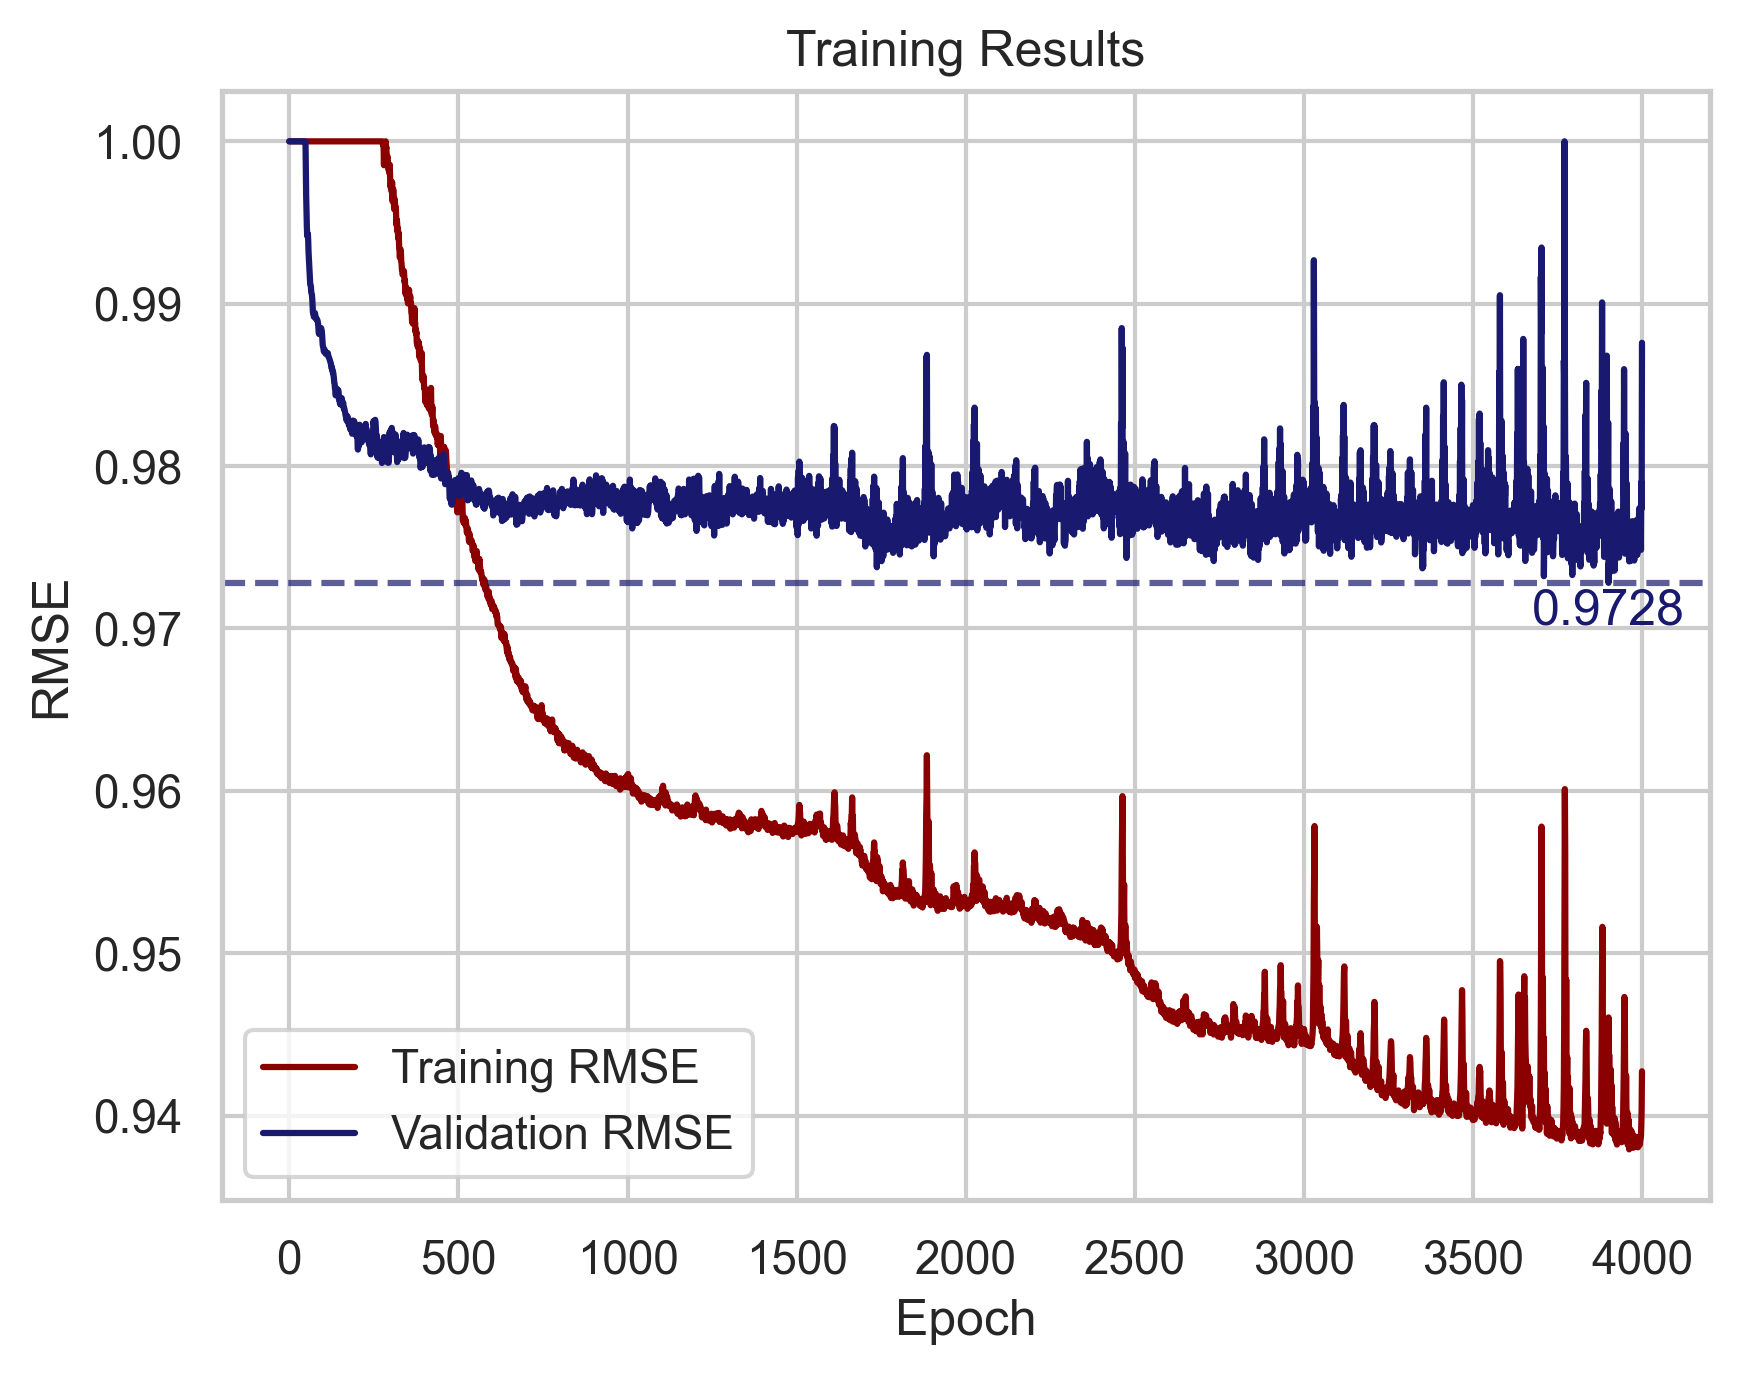
\includegraphics[width=0.7\linewidth]{image.png}
  \caption{Train run of the top performing model}
  \label{fig:top-model}
\end{figure}
\subsection{Baselines}

To assess the value our solution adds to the field of collaborative filtering, we compare it's performance against that of some standard models.

\subsubsection{Alternating Least Squares}

Alternating Least Squares (ALS) turns an otherwise quartic matrix factorization problem into one that is only quadratic by alternating between optimizing the user matrix while holding the item matrix constant and vice versa. When applied to the public test set, it achieved a RMSE score of 1.426

\subsubsection{Neural Collaborative Filtering}

Our Neural Collaborative Filtering (NCF) model is fairly vanilla. We used two embedding layers followed by a feed forward neural network. The ReLU activation function was used at all layers besides the final layer. We trained using the Adam optimizer with a learning rate of 0.001, MSE loss, and embedding dimension 16. After 25 epochs, this model achieved a RMSE score of 1.094 on the public test set.


\section{Discussion}
\label{sec:discussion}
\label{sec:tips-software}

The results of our experiments demonstrate the benefits and drawbacks of adapting the LightGCN architecture for use in collaborative filtering. Our findings indicate this approach is highly effective in predicting user ratings and is capable of outperforming baseline models such as ALS and NCF. 

The strength of LightGCNPlus is apparent. Even with only one layer, the model is capable of leveraging the interactions between neighbouring nodes to make accurate predictions as demonstrated by the singe-layer score in table \ref{table:results}. Adding more layers allows the model to capture further nuances in user-item rating relationships and increase performance, although more resources are required for training. Finally, averaging multiple trained models (ensembling) allowed us to increase performance even further. This demonstrates how leveraging the individual strengths of multiple models can improve overall performance.

Despite the impressive results achieved with LightGCNPlus, there are some limitations. The most obvious is the inherent complexity resulting from increasing model depth; higher layer counts are required for better performance but they come at the cost of greater training time and resource exependiture. Another drawback is model's sensitivity to the hyper parameters K, L, and C. While these parameters are powerful and can result in drastic performance improvement, they require a fair amount of experimentation and may limit the speed at which a LightGCNPlus model can be prepared for deployment. Finally, while ensembling does achieve better performance, it introduces another parameter to tune (number of models, M) and requires the training of multiple models. This again contributes to the overall complexity of the approach and may be a limiting factor in resource- or time-constrained settings.



\bibliographystyle{IEEEtran}
\bibliography{howto-paper}

\end{document}
